% !TEX ROOT = ersti.tex

an der Uni Heidelberg! Wenn ihr diese Ersti-Info in den Händen haltet, habt ihr euch wahrscheinlich dazu entschieden, hier Informatik, Mathematik oder Physik zu studieren -- herzlichen Glückwunsch zu diesem großen und wichtigen Schritt! Heidelberg ist eine wunderschöne Stadt und die naturwissenschaftlichen Fakultäten der Universität haben national und international einen hervorragenden Ruf. Auch das Verhältnis zwischen der Professorenschaft und den Studierenden ist in aller Regel überdurchschnittlich gut -- einem erfolgreichen, interessanten und lehrreichen Studium steht also nichts mehr im Wege. Dabei wünschen wir euch erstmal viel Spaß! \smiley

Da es erfahrungsgemäß vor allem am Anfang des Studiums trotzdem ein paar Probleme gibt, was die neuen Strukturen an der Uni, den Studienalltag und so wichtige Nebensächlichkeiten wie Wohnen, Finanzen, Ausgehen -- aber auch Soziales, Umwelt und Politik -- angeht, wollen wir als Fachschaft versuchen, euch mit dieser Info-Broschüre einige nützliche Tipps und Starthilfen für den Uni-Dschungel mit auf den Weg zu geben.

\vfill
\eject

Wir hoffen, dass alles Wichtige angesprochen wird. Falls ihr noch Fragen, Anregungen oder Kritik habt, könnt ihr euch jederzeit an uns wenden: einfach per Mail\footnote{fachschaft@mathphys.info} oder direkt persönlich im Fachschaftsraum 01.301 im Mathematikon.

Falls ihr euch jetzt fragt, wer oder was die Fachschaft eigentlich ist und was wir außer dem Ersti-Info noch alles machen, dann könnt ihr dies im Kapitel \hyperref[diefsmathphys]{Fachschaft MathPhysInfo} nachlesen. \\\\

\noindent Viel Spaß und Erfolg im Studium,\\\\

Eure Fachschaft MathPhysInfo


\begin{figure}[b]
\centering
% https://xkcd.com/1670/
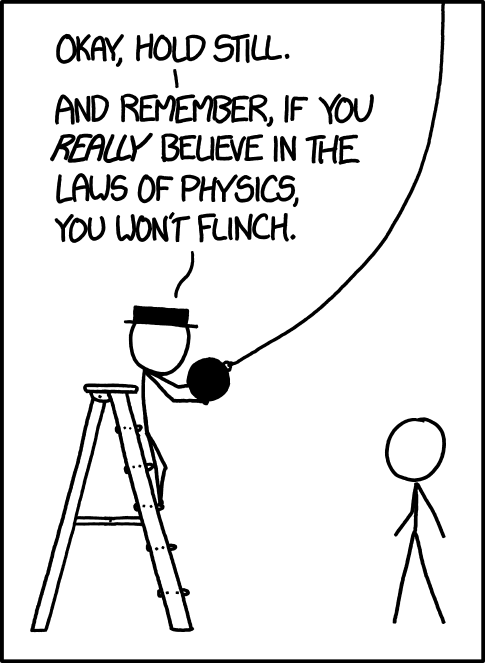
\includegraphics[height=8cm]{bilder/laws_of_physics_2x.png}
\end{figure}
